
\documentclass[a4paper, 10pt]{IEEEconf}  

\usepackage{geometry}
\geometry{a4paper, margin=1in}
  
  
\usepackage{subcaption}  
\usepackage[export]{adjustbox}    
\usepackage{verbatim}
\usepackage{graphicx}
\usepackage{pdfpages}
\usepackage{cite}
\usepackage{listings}
\usepackage{float}
\usepackage{url}
\usepackage{hyperref}
\usepackage{fancyhdr}
\usepackage{multicol}

\lstset{
	tabsize=2,
	breaklines=true
}

\setlength{\parskip}{1em}
\onecolumn

\title{\LARGE \bf Assignment 3: TensorFlow Neural Network Training\\Industrial Systems Design and Integration 282 772}
\author{Marc Alexander Sferrazza \\ 12164165
\thanks{This work was not supported by any organization}
\thanks{Faculty of Mechatronics Engineering, Massey University, Albany, Auckland, New Zealand
        {\tt\small Progress of project: https://github.com/alex1v1a/Industrial-Systems-Design-and-Integration} } }

\begin{document}

\maketitle
\begin{figure}[H]
  \begin{center}
  
\includegraphics[width=110mm]{images/tf}
  \label{fig:kinetic}
  \end{center}
\end{figure}
\thispagestyle{empty}
\pagestyle{plain}


%%%%%%%%%%%%%%%%%%%%%%%%%%%%%%%%%%%%%%%%%%%%%%%%%%%%%%%%%%%%%%%%%%%%%%%%%%%%%%%%

\begin{abstract}
In this documentation TensorFlow's neural network machine learning is used to find a function for y=f(x) given some inputs and outputs. The process involves using the Multi-Layered Perceptron (MLP) technique training and placeholders are used to provide input.
\end{abstract}


\clearpage
\thispagestyle{empty}
\tableofcontents
\begingroup
\let\clearpage\relax
\listoffigures
%\listoftables
\endgroup
%\thispagestyle{empty}
\clearpage
\twocolumn

%%%%%%%%%%%%%%%%%%%%%%%%%%%%%%%%%%%%%%%%%%%%%%%%%%%%%%%%%%%%%%%%%%%%%%%%%%%%%%%%
%%%%%%%%%%%%%%%%%%%%%%%%%%%%%%%%%%%%%%%%%%%%%%%%%%%%%%%%%%%%%%%%%%%%%%%%%%%%%%%%
\clearpage
\setcounter{page}{1}
%\thispagestyle{empty}
\onecolumn

\section{INTRODUCTION}

TensorFlow is a free(open-source) python language based library which is used for machine learning (intelligence) using neural networks to determine functions based on given inputs and outputs\cite{ML}. As TensorFlow (TF) is supported by the community it makes as a favourable tool to learn, and is not only capable of black box systems, but also able to coordinate with complex systems with learning nodes.

In this documentation the program TensorFlow is used to train a neural network that will approximate an unknown function of y=f(x) for a given vector. Using Python 3.5+ syntax and TensorFlow 1.0+ syntax, a predefined data set csv file will be called on which to preform the learning task for an output range.


%%%%%%%%%%%%%%%%%%%%%%%%%%%%%%%%%%%%%%%%%%%%%%%%%%%%%%%%%%%%%%%%%%%%%%%%%%%%%%%%

\subsection{Installation}

As TensorFlow uses Python, it supports multiple platforms including Mac, Windows, Linux, and Chrome OS. I have successfully installed Python 3.6 with a TensorFlow Python 3.5 CPU based workspace from source and have things compiled nicely; however for consistency with the lectures at Massey and to avoid any unnecessary errors I have completed these tasks using the advised programs with Visual Studio's CODE on Windows 10 OS\cite{CODE}. To setup and install TensorFlow simply follow the instructions on the TensorFlow website, or see the Getting Started with TensorFlow video on Frazer Nobles YouTube channel \cite{tfinstall}

When setting up TensorFlow it features to automatically add to the environmental variables PATH, however the Python version and must be set to 3.5 manually (due to current version of 3.6), along with the option for CPU or GPU compiling. Visual Studios CODE is installed as the editor with a built in terminal cmd for quick compiling. Finally after setting up and installing TensorFlow with Python and CODE, a test program is written to check the status of the install with success\cite{GS}.

\begin{figure}[H]
  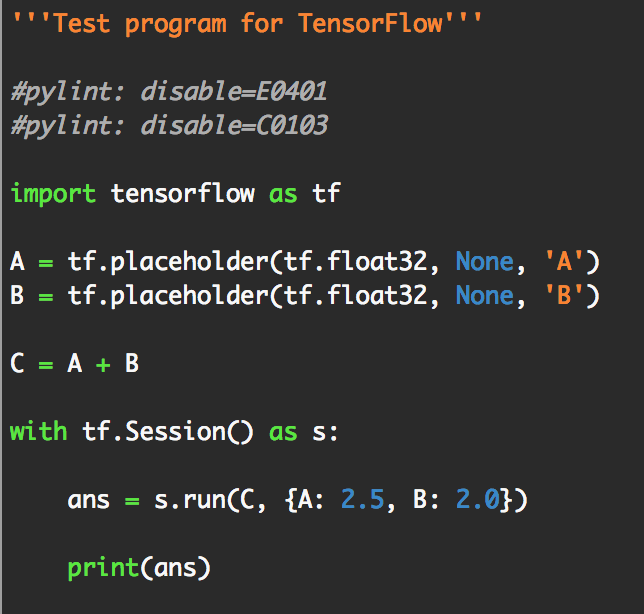
\includegraphics[width=0.5\linewidth, center]{images/test}
  \caption{Test file to check the working status for TensorFlow install, Result = 4.5}
  \label{fig:Test file to check the working status for TensorFlow install, Result = 4.5}
\end{figure}

%%%%%%%%%%%%%%%%%%%%%%%%%%%%%%%%%%%%%%%%%%%%%%%%%%%%%%%%%%%%%%%%%%%%%%%%%%%%%%%%
%%%%%%%%%%%%%%%%%%%%%%%%%%%%%%%%%%%%%%%%%%%%%%%%%%%%%%%%%%%%%%%%%%%%%%%%%%%%%%%%
%\clearpage
\section{METHOD}

Using TensorFlows neural network training MLP method, an approximation can be made for the y=f(x) function. As discussed in the lectures, the training method involves the input to segment blocks, where it is compared and examined with the relationship of output in a set shape space. The learning rate is the increment of which will define how well the relationship can be made with the smoothest function; this over iterations with a certain node size (mutations) and can give a higher accuracy with more reliable results of many iterations. 

%%%%%%%%%%%%%%%%%%%%%%%%%%%%%%%%%%%%%%%%%%%%%%%%%%%%%%%%%%%%%%%%%%%%%%%%%%%%%%%%
%\clearpage
\subsection{Nodes}

Nodes in a graph represent mathematical operations, while the graph's edges represent multi-dimensional data arrays (tensors); by combining Tensor nodes more complicated operations can be computed.

\begin{figure}[H]
  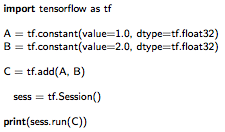
\includegraphics[width=0.35\linewidth, center]{images/nodes}
  \caption{laser plugin node setup}
  \label{fig:laser plugin node setup}
\end{figure}

Communicated between nodes can be compared to the action synapsis in the brain. When there is a slow learning rate, more iterations are required, but if there is a higher learning rate it will take a lot of time getting stuck in local minimums. The more nodes there are, the more variations there will be and the different types of variations the learning algorithm will try. For a three node two layer base there are 6 nodes total, adding the input and outputs give 8 nodes.

%%%%%%%%%%%%%%%%%%%%%%%%%%%%%%%%%%%%%%%%%%%%%%%%%%%%%%%%%%%%%%%%%%%%%%%%%%%%%%%%

\subsection{Multi-Layered Perceptron (MLP) Training}

Multi-Layered Perceptron (MLP) is a class of feedforward artificial neural network. There are at least 3 layers of nodes of which are neurons except for input nodes and are trained by weight and changing their connections after each piece of data is passed using back-propagation. \cite{MLP2}

Placeholders are used to provide input for the organisation of multiple layers. In many cases MLP's are used for solving problems stochastically such as complex problems that require more approximate solutions which makes it a powerful tool when used finding the function of a graph an performance based problems.

Using this training method for finding the function of f(x) utilises the regression technique and when preformed with the response variable being categorical can find the error of the output from the expected result, this is also known as supervised learning.

As such mentioned in the tutorial introduction for the basis of this task the nodes are arranged into layers as per below.

\begin{figure}[H]
  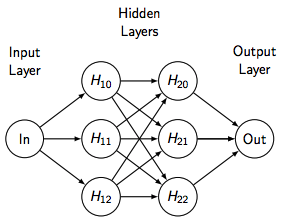
\includegraphics[width=0.5\linewidth, center]{images/mlp}
  \caption{A Multi-Layer Perceptron (MLP) neural network. Here, there are two
hidden layers, each with three neurons. The input and output layers have one
neuron each}
  \label{fig:A Multi-Layer Perceptron (MLP) neural network. Here, there are two
hidden layers, each with three neurons. The input and output layers have one
neuron each}
\end{figure}

%%%%%%%%%%%%%%%%%%%%%%%%%%%%%%%%%%%%%%%%%%%%%%%%%%%%%%%%%%%%%%%%%%%%%%%%%%%%%%%%
%\clearpage
\subsection{Importing the CSV}

A csv file, containing pairs of x and y values are read into the variables inputX and inputY respectively. In the lecture slides for machine learning part 2 it mentions several ways in which to import a csv file with the utilities library as utilise features = utils.read CSV(['./data/data.csv']) etc however this program will use the csv library mentioned in code. The values are read into the shaped array and appended to each line for the plots, there are 101 values total. 

After these values are read in the input is passed as places holders to the MLP which in turn uses two layers for the computation learning and parameters mentioned in the section above and the code attached in the appendix.

%%%%%%%%%%%%%%%%%%%%%%%%%%%%%%%%%%%%%%%%%%%%%%%%%%%%%%%%%%%%%%%%%%%%%%%%%%%%%%%%
%\clearpage
\subsection{Base Optimiser}

Initially the Gradient Computation optimiser was used as per the example in tutorial 4 example. While this produced fair results, they have room for improvement with this task. The Gradient Optimiser works by it's automatic differentiation, the chain rule knows the derivatives of each operation and can combine them automatically.

The Adam Optimiser is used to preform this optimisation. It provides better results and does this using a couple of methods including re-scaling of gradients, an automatic step size bound and annealing, and compensates for changes in f(x) over time. The stochastic function with parameters gives a better estimate for more complex situations and in turn can compensate for the unforeseen in a more reasonable state.

%%%%%%%%%%%%%%%%%%%%%%%%%%%%%%%%%%%%%%%%%%%%%%%%%%%%%%%%%%%%%%%%%%%%%%%%%%%%%%%%
%%%%%%%%%%%%%%%%%%%%%%%%%%%%%%%%%%%%%%%%%%%%%%%%%%%%%%%%%%%%%%%%%%%%%%%%%%%%%%%%

\section{RESULTS}

After successfully configuring the Multi-Layered Perceptron (MLP), reading in the values in the provided csv, preforming the learning task, the results can be shown below on an image illustrating the original data set and the inferred output of the program.

\begin{figure}[H]
  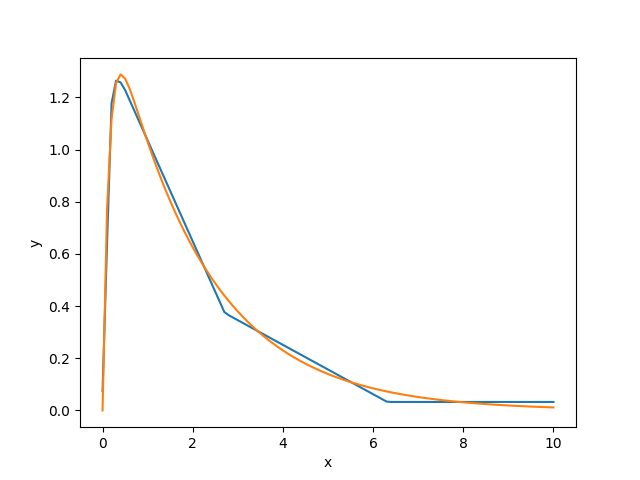
\includegraphics[width=0.8\linewidth, center]{images/plot}
  \caption{The final resultant is shown in compare on a graph}
  \label{fig:The final resultant is shown in compare on a graph}
\end{figure}

Once the initial results were found, to further the accuracy of the output the training of the MLP using the Adam Optimiser algorithm was used as suggested in class, please see variable for assigned learn rate in the code in the appendix. Below is the revised version using the Adam optimiser with specified nodes and learning rates as described in the logic documentation \cite{adam}. A clear difference between the optimiser reflects the accuracy for the learning of the function in this case.

\begin{figure}[H]
  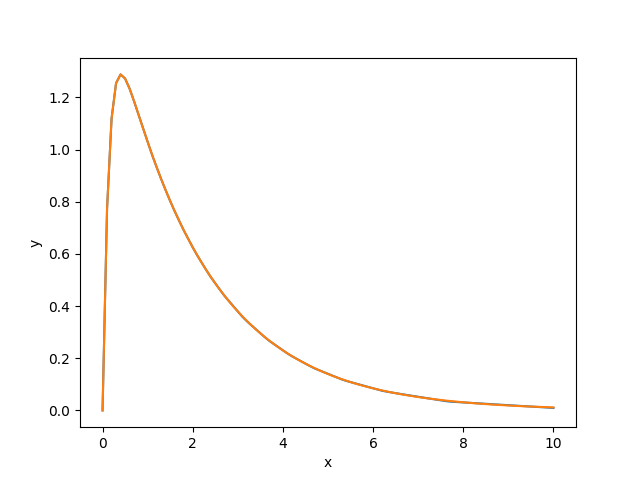
\includegraphics[width=0.8\linewidth, center]{images/3}
  \caption{The final resultant is shown in compare on a graph}
  \label{fig:The final resultant is shown in compare on a graph}
\end{figure}

The above figure was produced using a node size of 300, with an epochy of 300,000 and learning rate of 0.005

%%%%%%%%%%%%%%%%%%%%%%%%%%%%%%%%%%%%%%%%%%%%%%%%%%%%%%%%%%%%%%%%%%%%%%%%%%%%%%%%
%%%%%%%%%%%%%%%%%%%%%%%%%%%%%%%%%%%%%%%%%%%%%%%%%%%%%%%%%%%%%%%%%%%%%%%%%%%%%%%%

\section{OUTCOMES}

The machine learning task was completed with best results using MLP and the Adam Optimisation technique. The node size is optimal from 20+ with a learning rate less then 0.02 and epochy (iterations) are subjectible.

%%%%%%%%%%%%%%%%%%%%%%%%%%%%%%%%%%%%%%%%%%%%%%%%%%%%%%%%%%%%%%%%%%%%%%%%%%%%%%%%
%%%%%%%%%%%%%%%%%%%%%%%%%%%%%%%%%%%%%%%%%%%%%%%%%%%%%%%%%%%%%%%%%%%%%%%%%%%%%%%%

\section{CONCLUSIONS}

For any progress related to the report please see the public Github repo for alex1v1a or use the link in the cover page to be automatically redirected to this project. The repo provides all relative project information

I have come to a further understanding learned the fundamentals of TensorFlow's with nodes and tensors, and the use of such machine learning tools like Multi-Layered Perceptron using placeholders. This is a powerful tool and from a basic level of understanding is a strong aspect of machine learning processing, it is a great skill to learn. 

The appendix contains a full documentation of my modified version of Frazer Nobles GitHub Tutorial 4 - Unfortunately I was unable to use Tutorial 6 to complete this assignment after several attempts using Batching.

%%%%%%%%%%%%%%%%%%%%%%%%%%%%%%%%%%%%%%%%%%%%%%%%%%%%%%%%%%%%%%%%%%%%%%%%%%%%%%%%
%%%%%%%%%%%%%%%%%%%%%%%%%%%%%%%%%%%%%%%%%%%%%%%%%%%%%%%%%%%%%%%%%%%%%%%%%%%%%%%%

\nocite{*}
\bibliographystyle{ieeetr}
\bibliography{references}

%%%%%%%%%%%%%%%%%%%%%%%%%%%%%%%%%%%%%%%%%%%%%%%%%%%%%%%%%%%%%%%%%%%%%%%%%%%%%%%%
%%%%%%%%%%%%%%%%%%%%%%%%%%%%%%%%%%%%%%%%%%%%%%%%%%%%%%%%%%%%%%%%%%%%%%%%%%%%%%%%

\clearpage
\onecolumn
\section*{APPENDIX}
\begin{lstlisting}[language = Python]
# pylint: disable=C0413
# pylint: disable=C0103
# pylint: disable=E0401

import os
import tensorflow as tf # TesnorFlow Librarys
import csv # For csv importing etc
import matplotlib.pyplot as plt # For graphing and plotting etc

# Adjustable Values, Nodes, Learning Rate, and epochy 
nodeSize = 300 # More variation, more mutation
learnRate = 0.005 # Lower the learning rate the higher accuracy
iteration = 300000 # How many times it will go through - epochy

os.environ['TF_CPP_MIN_LOG_LEVEL'] = '3' # Suppresses warnings

# Import csv file, assign coloums as inputX, inputY respectivly, no determined allocation size for memory
inputX = [] 
inputY = [] 
# Open and read in data_set.csv
with open('data_set.csv','r') as csvfile: 
    plots = csv.reader(csvfile, delimiter=',') 
    for row in plots: 
		# Add each line of the csv to the row array for X and Y
        inputX.append([float(row[0])]) 
        inputY.append([float(row[1])])

# Placeholders are used, tensorflow diag 32 type with shape of nil, 1 - labeled x and y respectivly
x = tf.placeholder(dtype=tf.float32, shape=[None, 1], name='x')
y = tf.placeholder(dtype=tf.float32, shape=[None, 1], name='y')

# MLP
def mlp_layer(in_x, w_shape, b_shape):
    '''mlp_layer'''
	# Using the get variable function with the passed through same shapes and random initializer with no conditions
    W = tf.get_variable(name='W', shape=w_shape, dtype=tf.float32,
                        initializer=tf.random_uniform_initializer())
    b = tf.get_variable(name='b', shape=b_shape, dtype=tf.float32,
                        initializer=tf.random_uniform_initializer())
	# Assign the output of the added variables with shape b					
    out_y = tf.add(tf.matmul(in_x, W), b)
	# Return the addition of the layer as passthrough
    return out_y

# Layer 1 computation
with tf.variable_scope('layer_1') as vs:
    h = mlp_layer(x, [1, nodeSize], [nodeSize])
    h = tf.nn.relu(h)
    vs.reuse_variables()

# Layer 2 computation
with tf.variable_scope('layer_2') as vs:
    y_ = mlp_layer(h, [nodeSize, 1], [1])

# Loss value for the mean squared error
loss = tf.losses.mean_squared_error(y, y_)
# Training of the MLP using the Adam Optimizer as suggested in class, please see variaible for assigned learn rate
training = tf.train.AdamOptimizer(learning_rate=learnRate).minimize(loss)

# We must initalize the tensorflow with both global and local
init = [tf.global_variables_initializer(), tf.local_variables_initializer()]

# Begin the learing session after everything is setup and imported
with tf.Session() as s:
	# Run the initializer for the session
    s.run(init)

	# After evaluating the shape, this section was removed and shaped on the import of the csv
    # x1 = s.run(tf.reshape(inputX, [101,1])) 
    # y2 = s.run(tf.reshape(inputY, [101,1]))

	# Begin the loop for the function of the assigned iteration steps.
    for i in range(0, iteration, 1):
		# Start the training 
        l, _ = s.run([loss, training], feed_dict={x: inputX, y: inputY})

		# Only print the 10 cycles of iterations - epochy ~ 1st Jan 1970 lol...
        if i % (iteration/10) == 0:
			# Print the trained value..
            print(l)
	
	# Assign the learning points to use for the plot
    p = s.run(y_, {x:inputX}) 
	# Plot the learning points
    plt.plot(inputX,p) 
	# Plot the origional csv values
    plt.plot(inputX, inputY) 
	# Label Axis etc...
    plt.xlabel('x') 
    plt.ylabel('y') 
	# Show plot
    plt.show()
\end{lstlisting}

\end{document}
